\documentclass[../main.tex]{subfiles}
\begin{document}
\label{sec:ssloverview}
Before discussing previously proposed solutions to the problem we
identified in Section~\ref{sec:introduction}, we present here a
generic overview of SSL/TLS.

SSL/TLS supports a wide array of cipher suites, but they can be
roughly split into two categories: cipher suites that support forward
secrecy, and cipher suites that do not. Cipher suites that offer
forward secrecy are ones wherein a compromised long-term private key
does not allow an adversary to compromise previously eavesdropped,
stored sessions. SSL/TLS's session establishment mechanism differs
based on the category to which the cipher suite belongs. Our must
support the corresponding control flows. In this section we present an
abstraction of the SSL/TLS handshake that we used as a basis for our
system's design.

In general, regardless of the cipher suite used, SSL/TLS uses the
long-term private key to negotiate ephemeral keys for use in the
current session; hence, to secure the long-term private key, we need
to examine the session establishment mechanism. Roughly, SSL/TLS's
handshake can be split into four steps (this decomposition is
illustrated in Figure~\ref{fig:abshandshake}):

\begin{enumerate}
  \item \textbf{Contacting the server and establishing parameters for
    the session}. Specifically, the exchange of hello messages that
    include: the server's certificate(s), a list of cipher suites supported by
    each side (to determine which cipher suite is to be used for this session),
    \srandom, and \crandom. The random variables are required to derive the
    symmetric secret used for securing communications.
  \item \textbf{Asymmetric key exchange}: based on the cipher suite
    selected, the client and server determine the asymmetric keys that are
    to be used to exchange the symmetric keys for the session. This step
    is necessary in two scenarios:
    \begin{enumerate}
      \item When the client and server both possess public key
        certificates, and each entity wishes to verify the other's identity
        during the handshake: we do not consider this case due to its
        rarity. Generally, the client verifies the server's identity as part
        of the SSL/TLS handshake, and the server verifies the identity of the
        client via some other means, such as a username \& password.
      \item When the client and server select a cipher suite that offers
        forward secrecy: these cipher suites function by first exchanging an
        ephemeral asymmetric secret. This secret is then used in
        negotiating the symmetric secret.
    \end{enumerate} In all other cases, the server's asymmetric keys
    are used to negotiate the ephemeral symmetric secret.
  \item \textbf{Ephemeral symmetric key negotiation}: The client and
    server establish the symmetric secret that is used for the current
    session. The symmetric ephemeral keys are calculated as outlined
    below:

    \begin{enumerate}
      \item The \crandom, \srandom, and a value denoted
        \texttt{PremasterSecret} are combined together, through use of a
        pseudo-random function (PRF), to generate a value called the
        \texttt{MasterSecret}. The \texttt{MasterSecret} is a 48-byte number,
        and is computed using the method outlined here in all SSL/TLS cipher
        suites. In contrast, the \texttt{PremasterSecret} is a random value,
        established as part of this step, the derivation of which depends on
        the cipher suite used.
      \item The \texttt{MasterSecret} is then used to generate a key
        block. A session key block consists of:
        \begin{itemize}
          \item \texttt{server\_write\_key}: used by the server to
            encrypt outgoing payloads, and by the client to decrypt incoming
            payloads.
          \item \texttt{client\_write\_key}: used by the client to
            encrypt outgoing payloads, and by the server to decrypt incoming
            payloads.
          \item \texttt{server\_mac\_secret}: used by the server to
            compute a MAC over outgoing payloads, and by the client to verify the
            MAC over incoming payloads.
          \item \texttt{client\_mac\_secret}: is used by the client to
            compute a MAC over outgoing payloads, and by the server to verify the
            MAC over incoming payloads.
          \item \texttt{client\_initialisation\_vector(iv)}: is not a
            key, but a value used to initialise the symmetric cipher at the
            client, before invoking the encryption routine on outgoing payloads,
            and at the server, before invoking the decryption routine on incoming
            payloads.
          \item \texttt{server\_iv}: same as above, but used by the
            server before invoking the encryption routine on outgoing payloads,
            and by the client before invoking the decryption routine on incoming
            payloads.
        \end{itemize}
    \end{enumerate}
  \item \textbf{Verifying the integrity of the just-negotiated keys,
    completing the session establishment}: Both the server and the client
    use their \texttt{mac\_secret} to compute a MAC across the payloads
    exchanged in establishing the session. The resultant \textit{finished
    message} is encrypted using the just-negotiated keys. If both sides
    successfully verify the MAC, the handshake is complete and the session
    is established. If either side fails to verify the MAC, the session is
    terminated.
\end{enumerate}

\begin{figure}[H] \centering
  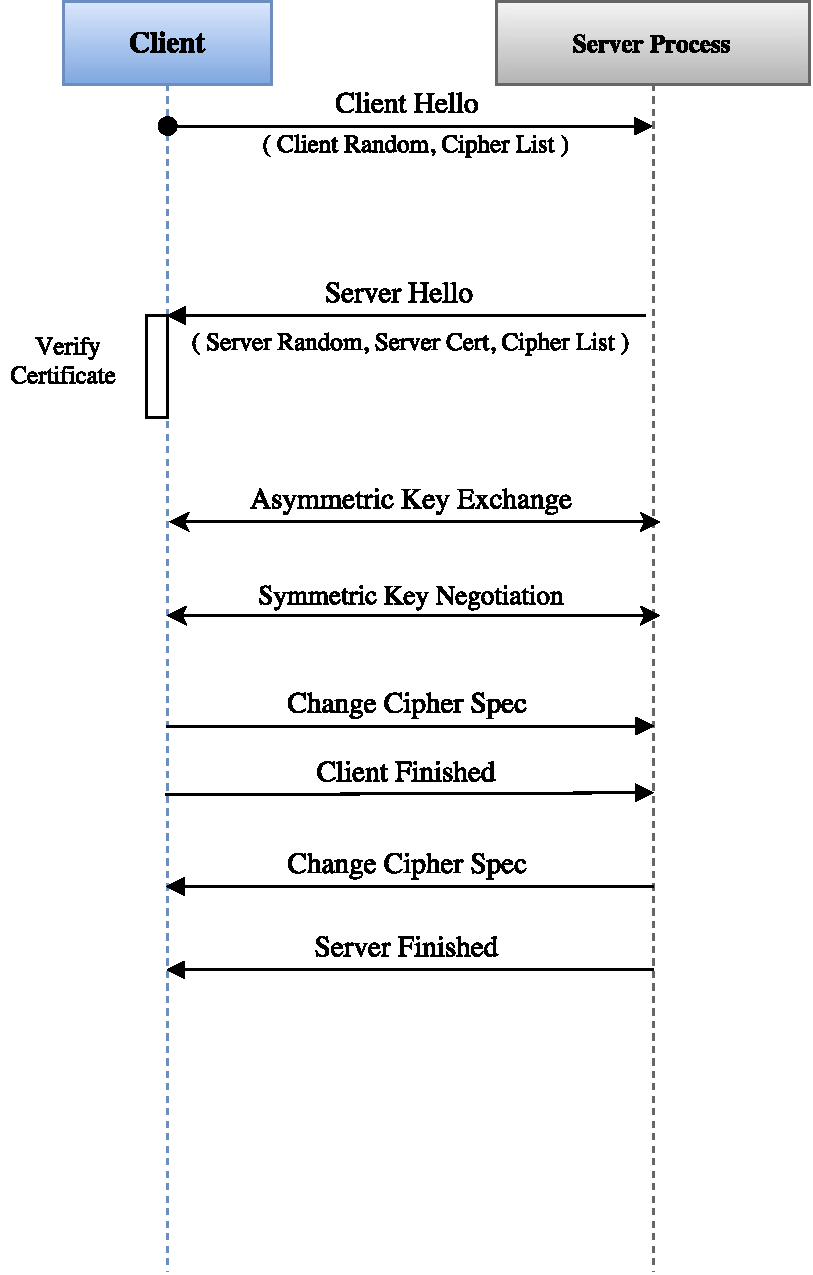
\includegraphics[scale=0.4]{images/abstract-handshake.pdf}
  \caption{SSL/TLS handshake generalization}
  \label{fig:abshandshake}
\end{figure}

\end{document}

%%% Local Variables:
%%% mode: latex
%%% TeX-master: "../main"
%%% End:
